

\tikzset{every picture/.style={line width=0.75pt}} %set default line width to 0.75pt

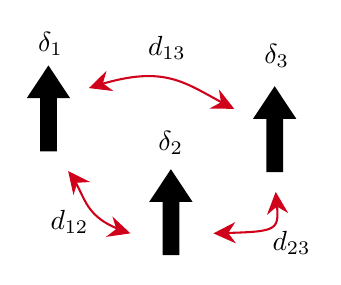
\begin{tikzpicture}[x=0.75pt,y=0.75pt,yscale=-1,xscale=1]
%uncomment if require: \path (0,300); %set diagram left start at 0, and has height of 300

%Up Arrow [id:dp8732081220560729]
\draw  [fill={rgb, 255:red, 0; green, 0; blue, 0 }  ,fill opacity=1 ] (11,45.33) -- (20.5,31) -- (30,45.33) -- (24.03,45.33) -- (24.03,71) -- (16.97,71) -- (16.97,45.33) -- cycle ;
%Up Arrow [id:dp6011286918484611]
\draw  [fill={rgb, 255:red, 0; green, 0; blue, 0 }  ,fill opacity=1 ] (70,95.33) -- (79.5,81) -- (89,95.33) -- (83.03,95.33) -- (83.03,121) -- (75.97,121) -- (75.97,95.33) -- cycle ;
%Up Arrow [id:dp7451953769890557]
\draw  [fill={rgb, 255:red, 0; green, 0; blue, 0 }  ,fill opacity=1 ] (120,55.33) -- (129.5,41) -- (139,55.33) -- (133.03,55.33) -- (133.03,81) -- (125.97,81) -- (125.97,55.33) -- cycle ;
%Curve Lines [id:da42525692800879833]
\draw [color={rgb, 255:red, 208; green, 2; blue, 27 }  ,draw opacity=1 ]   (31.84,83.56) .. controls (38.95,94.28) and (37.51,103.13) .. (57.4,110.13) ;
\draw [shift={(60,111)}, rotate = 197.49] [fill={rgb, 255:red, 208; green, 2; blue, 27 }  ,fill opacity=1 ][line width=0.08]  [draw opacity=0] (10.72,-5.15) -- (0,0) -- (10.72,5.15) -- (7.12,0) -- cycle    ;
\draw [shift={(30,81)}, rotate = 51.91] [fill={rgb, 255:red, 208; green, 2; blue, 27 }  ,fill opacity=1 ][line width=0.08]  [draw opacity=0] (10.72,-5.15) -- (0,0) -- (10.72,5.15) -- (7.12,0) -- cycle    ;
%Curve Lines [id:da4089633773753214]
\draw [color={rgb, 255:red, 208; green, 2; blue, 27 }  ,draw opacity=1 ]   (103.47,110.9) .. controls (132.46,110.07) and (131.79,109.99) .. (130.27,93.96) ;
\draw [shift={(130,91)}, rotate = 445.16] [fill={rgb, 255:red, 208; green, 2; blue, 27 }  ,fill opacity=1 ][line width=0.08]  [draw opacity=0] (10.72,-5.15) -- (0,0) -- (10.72,5.15) -- (7.12,0) -- cycle    ;
\draw [shift={(100,111)}, rotate = 358.33] [fill={rgb, 255:red, 208; green, 2; blue, 27 }  ,fill opacity=1 ][line width=0.08]  [draw opacity=0] (10.72,-5.15) -- (0,0) -- (10.72,5.15) -- (7.12,0) -- cycle    ;
%Curve Lines [id:da6145675949482681]
\draw [color={rgb, 255:red, 208; green, 2; blue, 27 }  ,draw opacity=1 ]   (43.37,39.9) .. controls (77.59,29.07) and (86.43,38.94) .. (107.64,49.81) ;
\draw [shift={(110,51)}, rotate = 206.24] [fill={rgb, 255:red, 208; green, 2; blue, 27 }  ,fill opacity=1 ][line width=0.08]  [draw opacity=0] (10.72,-5.15) -- (0,0) -- (10.72,5.15) -- (7.12,0) -- cycle    ;
\draw [shift={(40,41)}, rotate = 341.27] [fill={rgb, 255:red, 208; green, 2; blue, 27 }  ,fill opacity=1 ][line width=0.08]  [draw opacity=0] (10.72,-5.15) -- (0,0) -- (10.72,5.15) -- (7.12,0) -- cycle    ;

% Text Node
\draw (20,98.4) node [anchor=north west][inner sep=0.75pt]  [font=\normalsize]  {$d_{12}$};
% Text Node
\draw (127,108.4) node [anchor=north west][inner sep=0.75pt]  [font=\normalsize]  {$d_{23}$};
% Text Node
\draw (67,14.4) node [anchor=north west][inner sep=0.75pt]  [font=\normalsize]  {$d_{13}$};
% Text Node
\draw (14,12.4) node [anchor=north west][inner sep=0.75pt]    {$\delta _{1}$};
% Text Node
\draw (72,60.4) node [anchor=north west][inner sep=0.75pt]    {$\delta _{2}$};
% Text Node
\draw (123,18.4) node [anchor=north west][inner sep=0.75pt]    {$\delta _{3}$};


\end{tikzpicture}
